% %This is a very basic article template.
% %There is just one section and two subsections.
\documentclass[authoryear, review,12pt,number]{elsarticle}
\usepackage[numbers]{natbib}
\usepackage{citep}
\usepackage{graphicx}
\usepackage{float}
\usepackage{rotating}
\usepackage{stfloats}
\usepackage{lineno}
\usepackage[linesnumbered,ruled,vlined]{algorithm2e}
\usepackage{tabulary}
\usepackage{graphicx}
\usepackage{color}
\usepackage[none]{hyphenat}
\usepackage[table]{xcolor}
\sloppy
\begin{document}

\begin{frontmatter}
\linenumbers
\title{Automated Classifying of EUNIS Habitats with Ontologies and Data Mining
methods}


\author[TUB]{T. Niklas Moran\corref{cor1}}
\ead{niklasmoran@mailbox.tu-berlin.de}

\author[TUB]{Simon Nieland}
\author[TUB]{Birgit Kleinschmit}

\author[TUB]{Michael F\"orster}

\address[TUB]{Geoinformation in Environmental Planning Lab, Technische
Universit\"at Berlin, Stra\ss e des 17. Juni 145, 10623 Berlin, Germany}

\cortext[cor1]{Corresponding author at: Geoinformation in Environmental Planning
Lab, Technische Universit\"at Berlin, Stra\ss e des 17. Juni 145, 10623 Berlin,
Germany. Tel.:+49 30 314 72601;}
\begin{abstract}
Write some text here..
\end{abstract}

\begin{keyword}
remote sensing, biotope classification, data mining,
generalisation, nature conservation, NATURA 2000, OWL2
\end{keyword}

\end{frontmatter}

\linenumbers

\section{Introduction - Context and Background}
% NATURA2000 obligations and local obligations = NATFLO
Recognizing that human-caused habitat destruction plays a dominant role in
biodiversity loss, the European Union has implemented an environmental
conservation framework to halt biodiversity loss in accordance with the
Convention on Biological Diversity (CBD, 2005). An integral part of this
framework is the EU Habitats Directive (Council Directive) 92/43/EEC [1992],
which established the Natura 2000 network of habitats. The law requires
conservation and monitoring of designated habitats by member states and for a
report to be submitted every six years. Due to these obligations and other
environmental and spatial planning requirements, the German federal state of
Rhineland-Palatinate started to implement a thematically integrated
state-wide system with all relevant geo-data for plans and decision-making at
all levels of government called NATFLO (Landscape objects from remotely
sensed data for nature conservancy). The semantic and thematic interoperability
effortlessly incorporates expert knowledge and helps decision-makers, scientists
from different disciplines and planners successfully communicate using
objective environmental data. To 
%% automated map-making
Since collection of comprehensive,
good-quality environmental data through field recordings is expensive and time
consuming, remote sensing and other technologies can potentially reduce costs
and provide a more robust data source that can be used in different domains. The
NATFLO project harnesses vector objects with various indicies in automated
workflows to allow for (semi) automated mapping. % (corbane et al 2015)
\subsection{NATFLO}
% do I need to describe the project?!

%% redundant:
As a result the federal authorities in Rhineland-Paltinate started to implement
such a system in mid-2014 under the name NATFLO . One of the goals of the projects is
multifunctionality which entails differing semantic conceptualizations. The use
of ontologies and ontology-based reasoning over vector objects was seen as the
solution to this problem. Using ontologies with the help of experts allows for
the translation from the Rhineland-Palitinate biotope system to the EU-wide EU
Nature Information System (EUNIS). Ontologies also allows
for comparison between areas with differing semantic conceptualizations and a
reasoning over objects. 

Yet as Lucas et. al (2015) point out there are no standards for classifying
habitats with Earth Observation (EO) data that can be applied to all sites. 

Due to differing standards and approaches of the various nature conservation
agencies in collecting and disseminating information, data comparison is
difficult. Different data types and data sources increase the difficulty in
comparing data from one site to another. Furthermoe, habitat monitoring can
be labor intensive and subjective.

Luckily, EO data could help reduce the burden of environmental monitoring and
also provide information on conservation status.

We propose an automated system that can classify Natura 2000 habitats
accoding to the EU-wide biotope classification schema called the European Union
Nature Information System (EUNIS) using EO data, an existing biotope map and
expert knowledge formalized in an ontology. The biotope data serves as class
labels for training a data mining algorithm.

\section{State of Research and Research Question}
Remote sensing has a rich history in environmental conservation, meteorology,
climate science and other fields. Due to this history remote sensing experts
have become very good at analyzing remote sensing data. Yet, remote sensing
image analysis implicitly incorporates the expertise and knowledge of the
individual performing the analysis and reduces objectivity. This can be divided
into remote sensing knowledge (spectral signature, remote sensing index, etc.)
and field knowledge (feature properties, spatial relations, etc)
\citep{Andres2013a}. This knowledge is often neither completely nor explicitly
defined but influences the classification. Thus, two experts can interpret the
same image differently due to their unique conceptualizations and experiences.
Further complicating matters, the classification chain is not documented and
controlled, reducing comparability and hindering attempts to reproduce the
results\citep{Arvor2013}. Therefore automated methods for remote sensing
classifications that produce accurate and reproducible results are desired.
An automated system would also reduce the time needed to analyze large
remote sensing datasets. Many approaches have been used to create an accurate
automated classification tool using statistics and different algorithms
from machine learning and data mining. Unfortunately most of these approaches
rely on experts to produce rule-sets or manually select training points. The
former relies on \emph{a priori} knowledge while the latter can be
time-consuming.
Neither are observation-based. There are many different automatic methods
for feature selection. A brief overview explaining the most common methods is
described below.

\subsection{Background - Remote Sensing and Ontologies}

\subsection{Feature selection}
%% focus on ML?

There are many different classification approaches with varying degrees of
complexity and requiring different levels of user input. One commonly used
classification approach, the maximum likelihood classification (MLC) approach,
among the most popular, has been used to study land use change in China
\citep{Ding2007}, analyze forest cover in Haiti \citep{Churches2014} and land
cover and land-use change in Egypt \citep{Shalaby2007}. Recent research suggests
support vector machines (SVMs) when compared to decision trees (DTs), a neural
network classifier and the MLC, produces better results \citep{Huang2002}. One
such DT is the ``Random Forest'' algorithm which has been shown to be better
than Adaboost \citep{Chan2008} and performed well when applied to the Cape Cod
National Seashore for coastal dune and salt marsh classification
\citep{Timm2012}.
% need more?

\subsection{Selection of Algorithm - SEaTH and Decision Trees}
We first chose the Separability and Thresholds
(SEaTH) \citep{Nussbaum2006} algorithm to automatically derive features important
for classification from the data because it is able to generate rules with
thresholds that can easily be transferred to an ontology. Saving the rules in
the ontology makes it clear what rules were used for classification and can be
used by experts to modify the rules to be more accurate. To compare
classification accuracy we selected the scikit-learn python suite
\citep{scikit-learn} due to its maturity and ease of use and the availability of
different algorithms. We settled on the ``DecisionTreeClassifier'' as one can
visualize the results and parse the tree to load the results into the ontology.
Moreover, an automated system should be able to use other algorithms as they become available.

\subsection{SEaTH} The Separability and Thresholds (SEaTH) algorithm
\citep{Nussbaum2006} statistically identifies characteristic features and their thresholds. It has
been used on remote sensing data for land cover classification \citep{Gao2011}
and nuclear installation classification \citep{Nussbaum2006}.
Using training data, the algorithm determines the separability of the object
classes and then calculates the thresholds for which the maximum separability
can be achieved using the given features. One benefit of the algorithm is that
one does not need many training objects.
In the Nussbaum, Niemeyer and Canty (2006) paper, for example, the authors
suggest using only very characteristic features for training and only used
around 10 samples per class\citep{Nussbaum2006}. The authors also state that
usually two features per class is enough to produce accurate results. Combining
this algorithm with an ontology would produces traceable results that are easy
to understand. This approach would also help fill the observation-based ontology
research gap as first described by Janowicz (2012) \citep{Janowicz2012}.

\subsection{Comparison with Decision Tree Classifier}
The decision tree classifier implemented in scikit-learn is a modified
classification and regression tree (CART)\citep{scikit-learn}. To minimize the
ruleset and reduce computation time, dimension reduction was performed on the
data using

\subsection{Semantic-based image interpretation}
Different fields (medical imaging, security, etc.) have used ontologies for
improving image retrieval and object detection. Only recently have ontologies
been adopted in remote sensing research. An ontology, defined as ``an explicit
specification of a conceptualization'' \citep{gruber1993} could help bridge the
semantic gap and allow for better data interoperability, workflow management and
automatic image interpretation \citep{Arvor2013} \citep{Andres2013a}. The term
``semantic gap'' refers to the difference between the higher-level descriptions
by experts and what can be extracted from the visual data. Remote sensing and
field expert knowledge can be digitized in ontologies, thus allowing for a
hierarchy of concepts for improved automatic image annotation and retrieval
using concepts from both fields to produce more accurate results
\citep{Srikanth:2005:EOA:1076034.1076128}. Janowicz \citep{Janowicz2012}
advocates for more observation-driven ontologies and for including machine
learning, geostatistics and data mining to construct ontological primitives.
Research on using observation-based ontologies for classifications is still
lacking. There are initiatives to use ontologies in biodiversity research. Below
are some examples.
\subsection{Ontologies in remote sensing research}
One such research project is the EU-funded ``Biodiversity Multi-Source
Monitoring System:
From Space To Species'' (BIO\_SOS) which seeks to develop tools to monitor and
map protected areas in the EU and uses ontologies modeled on the Land Cover
Classification System (LCCS) and the General Habitat Category (GHC) to achieve
this goal \citep{Arvor2013}. Using the taxonomy of the different classification
systems allows expert knowledge to be included in the process.
Further work as part of the project includes creation of a standardized
framework for habitat monitoring and mapping called the Earth Observation Data
for Habitat Montioring (EOD-HAM) system \citep{Lucas2015}. The system harnesses
knowledge from both remote sensing and ecology to classify Natura 2000 sites
using a hierarchical classification system. The EOD-HAM system uses both
pixel-based analysis and OBIA for greater classification accuracy but still
relies on a rule-base created by an expert or the user. Other research includes
a semi-automatic semantic classification approach for urban building types using
a three-layered architecture was developed by di Sciascio et al.\ which showed
promising results \citep{diSciascio2013}. Belgiu et al. \citep{Belgiu2014} used
Airborne Laser Scanning (ALS) data and empirically determined thresholds using
the Random Forest (RF) classifier to perform an ontology-based classification of
building types. Forestier et al. \citep{Forestier2012470} used an ontology to
classify pre-segmented regions using a knowledge-base. Sheeren et al.
\citep{Sheeren2006ML} developed a method to automatically acquire classification
rules using a newly developed genetic programming algorithm.
Sheeren et al.\ also used the data mining algorithm C4.5 for automatic rule
generation with satisfactory results. Nieland et al. \citep{Nieland2015}
demonstrated the potential for ontological inference and hierarchical
matchmaking as a way to improve spatial data interoperability. An automated
image analysis and classification process that could be applied to the whole
Natura 2000 network would be ideal and allow for comparison between habitats.
Such an automated tool could combine the benefits of object-based image analysis
(OBIA) with linguistic terms for a traceable and reproducible classification
system. When an ontology is available, scientists can follow how the classes
were developed and become aware of possible incompatibilities before combining
datasets \citep{Janowicz2012}.

\section{Method}
\subsection{Expert Knowledge and Data Mining}
We chose supervised classification algorithms that are able to exploit expert
knowledge, perform classification tasks quickly and accurately and produce human
understandable rule sets for further scrutiny and refinement. Therefore, the
SEaTH algorithm and the Decision Tree algorithm (a type of classification and regression
tree) were selected to find the optimal combination of environmental indices and
object properties that differentiate between objects. The labels used to
differentiate between polygons come from the Rhineland Palatinate biotope map
last updated in 2015. Consulting with experts, the translation between the
Rhineland-Paltinate (OSIRIS) biotopes and EUNIS was possible. The properties of
the EUNIS biotopes was then given to each polygon of the segmented data that fit
within the biotope boundary. The 
% Nieland, Kleinschmit, F\'orster 2015
\subsection{Ontology-based Reasoning}
Both the data mining algorithms, SEaTH and Decision Trees can produce rule
set with defined thresholds that can be chained together with logical operators
(AND, OR, NOT) that then can be imported into an OWL ontology. Once in an
ontology, a reasoner can perfrom A-Box reasoning. The reasoner chosen for its
speed and efficiency is the Fact++ Reasoner.

A benefit of using ontologies is that one can have hierarchies of concepts and
the reasoner can find logical inconsitencies and subsumption of concepts.
\subsection{Stereo Matching Based DSM}
The ASCII point data has a resolution of 0.5m which was rasterised using IDW.
\subsection{LiDAR DTM}
The LiDAR ASCII point clouds were acquired between 2003 and 2009 and contain
first and last pulse. The data contains on average 4 points per m$^{2}$ and
this was rasterised with IDW.
%

\subsection{Environmental Data}

9 Segmentation Classes from ecognition:
'BodenOffen', 'BodenVegKarg', BodenVegMittel', 'BodenVegSchwach',
'BodenVegStark', 'NoVeg', NoVegHoch', 'Plantagen', 'Veg'

\subsection{Study Area and Data}
The study area is located in the southeastern part of the Trier-Saarbug district
in the federal state of Rhineland-Palatinate, Germany. At approximately
200km$^{2}$, Luxembourg borders the district to the west and the federal state
of Saarland to the South.
\begin{figure}
	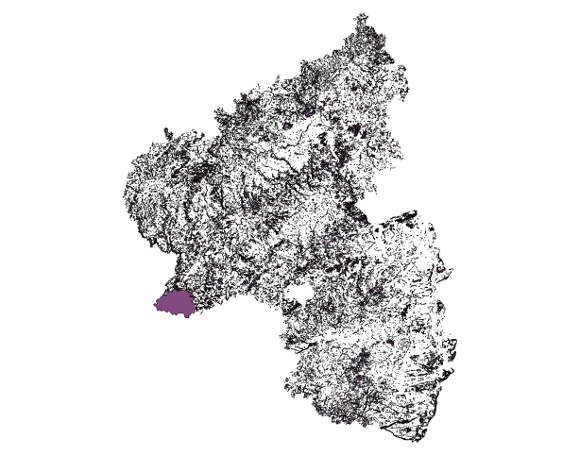
\includegraphics[width=\textwidth]{diagrams/study_area_small.png}
\end{figure}

\subsection{Data and Preprocessing}
All input data comes from the RLP Ordnance Survey (Landesamt f\"ur Vermessung und
Geobasisinformation).



The data is segmented by RLP AgroScience using
multispectral (B, G, R, NIR) orthophotos with a 0.2m ground resolution and a
2 x 2km tile size that are produced every 2 years. The iterative object-based
image analysis is performed using eCognition Server and segments
the data using thresholds and multiresolution approaches (Baatz and
Sch\'ape 2000). The segmentation process uses information solely from aerial
images based on spectral information (NDVI and Bare Area Index) and height
(Tintrup gen. Suntrup et al. 2015). Further indicators 

\begin{itemize}
    \item Clip the biotope map to the extent of Saarburg-Trier
    \item Join EUNIS properties to OSIRIS class names
    \item Postgis join using ST\_WITHIN to select segmented polygons completely
        within biotope map polygons
    \item Join zonal statistics to the segmented polygons
\end{itemize}
Since this study focuses on the the area of Saarburg-Trier, the first step was
to clip the biotope map with the extent of Trier-Saarburg. Then we join a table
that has been created with the help of ecologists in Rhineland-Paltinate that
translates the OSIRIS biotopes to the corresponding EUNIS biotope class. We then
perform a spatial join using Postgis ST\_WITHIN to select the segmented polygons
that lie within the biotope map. These polygons have all the biotope information
attached to them and in the final step have the zonal statistics with
morphological and hydrolgical (SAGA wetness index, ) and topographic indicies (topographic wetness
index, )
After joining EUNIS characteristics to the RLP biotope map, the map was 
spatially joined with the pre-segmented remote sensing data. Defiens eCognition
software was used for the segmentation and was performed by RLP AgroScience. 

The remote sensing data already had zonal statistics computed for all of the
polygons. A list of the zonal statistics are below.

% Future segmentation processes will incorporate DTM derived indicies and satellite imagery.

We apply a PostGIS spatial join query using ST\_WITHIN to select only those
polygons from the segmented dataset that fall completely within the biotope polygon of our preprocessed
biotope map. We join those polygons
with EUNIS characteristics and also attach zonal statistics that are calculated
for every polygon. The last step in the pre-processing workflow is the
replacement of NULL values with zeros. The null values arise due to small
polygon sizes created by the segmentation process. In the future, a new
segmented dataset that respects the biotope boundaries should be available and
will reduce the problems from selecting polygons that fall completely within the
polygon.


\subsection{Training/Testing Dataset}
To create a training data, we randomly select 200 training objects per class. A
subset of these objects, 20 per class, are used as input for the SEaTH
algorithm as it performs better with fewer characteristic objects.


\subsection{Results}

We were able to reach over 90\% accuracy for dry and aquatic classes using the
decision tree classification algorithm from sci-kit learn. The same results
using the 13 most important features produced by the random forest algorithm
also achieved equal results. This can potentially reduce the amount of features
and statistics that need to be calculated to classify habitat objects. This
would greatly reduce computation and storage requirements for habitat
classification.

\section{Discussion}
SEaTH shows much better separability when one chooses larger objects and fewer
training objects per clas. Training SEaTH on a few carefully selected objects
being ideal class representations further increases the separability, but the classification
accuracy suffers when applied to the complete data set. Thus, SEaTH appears to
overfit. Using two sets of rules produced from different sized training data
produced quite different results when tested on the same dataset.

The next step is to use the base wetness classes and combine them with other
EUNIS class properties to be able to classify biotopes throughout Europe. This
would allow for comparison and increase scrutiny of existing biotope maps.

\section{Conclusion}
We showed an automated workflow using ontologies and data mining algorithms can
accurately classify wetness. Moreover, the use of ontologies if published on the
Internet can allow otehrs to reuse the owrkflow and make their own
modifications.
\bibliographystyle{model2-names}
\section{References}
\bibliography{references}
\end{document}
